\section{Theorie}
\label{sec:Theorie}

Bei der TSDC (Thermally stimulated depolarization current) werden Dipole in einem kalten Ionenkristall erzeugt
und der entstehende Strom $I$ beim Aufwärmen gemessen. Über den Verlauf des Stromes $I$ in Abhängigkeit von der Temperatur $T$
 lassen sich Aussagen über die Aktivierungsenergie $W$ und schlussendlich über die Relaxationszeit $\tau$ treffen.

\subsection{Ionenkristalle}
Ordnen sich Anionen und Kationen in einer regelmäßigen Kristallstruktur an, spricht man von Ionenkristallen.
Die Bindungskraft ist die elektrostatische Anziehungskraft zwischen den involvierten Ionen, eine sehr starke Kraft, weshalb die Schmelzetemperatur 
von Ionenkristallen sehr hoch ist \cite{schmelzpunkt}.

In Ionenkristallen gibt es verschiedene Defekte. So kann eine Gitterstelle unbesetzt sein, mit einem Fremdatom besetzt sein oder es können Zwischengitterplätze belegt sein, schematisch zu sehen in
\autoref{fig:defekte}.

\begin{figure}[H]
    \centering
    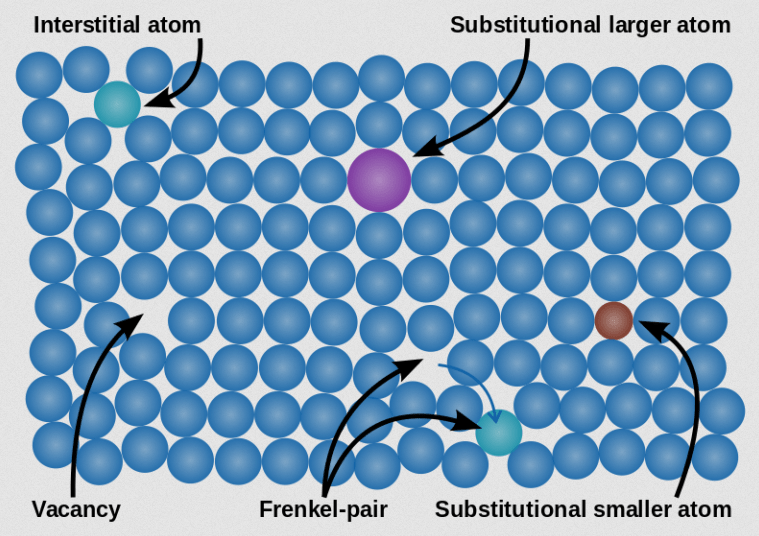
\includegraphics[width=0.85\textwidth]{Bilder/bildd.png}
    \caption{Schematische Darstellung von Defekten in Kristallstrukturen \cite{bild}.}
    \label{fig:defekte}
\end{figure}

Ein idealer Kristall besteht zwar aus geladenen Teilchen, aber die Verhältnisse der Ladungsträger sorgen dafür, dass der Kristall
insgesamt nach außen hin elektrisch neutral ist.

Wird nun ein Fremdatom mit einer anderen Ladung $q_i$ in das Gitter eingeführt, beispielsweise ionisiertes Strontium mit einer zweifach positiven Ladung in ein Cäsium-Iodid-Kristall, wo das Cäsium nur einfach positiv geladen ist,
dann ist der Kristall lokal um das Strontium positiv geladen. Um für die zweifache positive Ladung zu kompensieren, kommt es zu Veränderungen innerhalb des Kristalls, z.B. durch die Verschiebung von Cäsium oder Iodid, sodass der Kristall
elektrisch neutral wird. Dabei entstehen Dipole $\vec{p}_i$ zwischen dem Strontium und den Cäsium-Leerstellen oder den verschobenen Iodid-Atomen. Diese Dipole sind bei Raumtemperatur zufällig verteilt, sodass der Kristall ein gesamtes Dipolmoment von 0 hat,
\begin{equation*}
    \vec{p} = \sum_i \vec{p}_i = \sum_i q_i \cdot \vec{r}_i = 0,
 \end{equation*}
 dabei ist $\vec{r}_i$ der Abstand der Ladungsträger in den einzelnen Dipolen.




\subsection{Dipolrelaxation}

Wird ein elektrisches Feld $\vec{E}$ angelegt, können sich diese Dipole rotieren. Gemäß
\begin{equation*}
    E_\text{pot} = - \vec{p} \cdot \vec{E}
\end{equation*}
ist die energetisch günstigste Orientierung erreicht, wenn die Dipole parallel zum Feld liegen. Dies ist nur unter der Anwesenheit eines elektrischen Feldes der Fall.
Die Orientierung der Dipole kann nun festgehalten werden, wenn man den Kristall stark kühlt. Wird das elektrische Feld nun ausgeschaltet, benötigen die Dipole eine gewisse Energie $W$, genannt Aktivierungsenergie, um das Coulomb-Potential des Ionengitters zu überwinden
und die nun energetisch günstigere zufällige Orientierung anzunehmen. 
Von Interesse ist dabei die Zeit $\tau$, die vergeht, bis der Kristall wieder entpolarisiert ist. Aufgrund der thermischen Natur lässt sich dieser Vorgang mit der Arrhenius-Gleichung \cite{fuller}
\begin{equation}
    \tau\left(T\right) = \tau_0 e^{\frac{W}{k_\text{B}T}}
    \label{eq:arrhenius}
\end{equation}
beschreiben. Die sogenannte Relaxationszeit $\tau\left(T\right)$ hängt dabei von der Aktivierungsenergie $W$ und der Temperatur $T$ ab. Weiterhin ist $\tau_0$ die charakteristische Relaxationszeit des Materials und $k_\text{B}$
die Boltzmannkonstante. Bei hohen Temperaturen strebt der exponentielle Faktor gegen $1$ und die Relaxationszeit wird zur charakteristischen. Bei niedrigen Temperaturen wird derselbe Faktor sehr groß und die Relaxationszeit nimmt exponentiell zu.
Anschaulich bedeutet das, dass die Wahrscheinlichkeit, aus thermischen Fluktuationen genug Energie zu kriegen, um die Aktivierungsenergie zu überwinden, bei niedrigen Temperaturen sehr klein ist und die mittlere Zeit, bis ein Dipol seine Orientierung ändert, entsprechend wächst.

Wird die kalte, polarisierte Probe nun mit einer konstanten Heizrate $b$ erwärmt, erhalten die Teilchen mehr Energie. Mit dieser Energie können sich unter anderem einzelne gebundene Ladungsträger aus Unreinheiten lösen (Trapped Charges), wenn sie
das bindende Potential überwinden können. Viel prominenter aber ist die Reorientierung der Dipole, sobald diese ihre Aktivierungsenergie $W$ erhalten. Diese Reorientierung (und zum kleinen Teil die nun freien Ladungsträger) in energetisch günstigere Zustände
sorgen für einen messbaren Strom, dem Depolarization Current.

Der Depolarization Current lässt sich über folgenden Gedanken quantifizieren \cite{fuller}:
\begin{equation*}
    I\left(T\right) \propto \left(\text{Polarisation pro Dipol}\right) \cdot \left(\text{Anzahl teilnehmender Dipole}\right) \cdot \left(\text{Dipolrelaxationsrate}\right)
\end{equation*}
Die Dipolrelaxationsrate ist das Inverse der Relaxationszeit \ref{eq:arrhenius}. Die Polarisation pro Dipol $P$ lässt sich über die Debye-Theorie schreiben als
\begin{equation}
    P = \frac{\vec{p}^2 \left\lvert \vec{E} \right\rvert}{3 k_\text{B} T}.
    \label{eq:polarisation}
\end{equation}
Die Anzahl teilnehmender Dipole $N\left(T\right)$ lässt sich bestimmen über
\begin{equation}
    N\left(T\right) = N_\text{p} \exp\left(\frac{-1}{b\tau_0} \int_{T_0}^{T} \exp\left(\frac{-W}{k_\text{B}T'}\right)\mathrm{d}T'\right),
    \label{eq:dipolanzahl}
\end{equation}
wobei $N_\text{p}$ die Anzahl ursprünglich parallel orientierter Dipole ist und $T_0$ die Starttemperatur, $T$ die Temperatur zu einem bestimmten Zeitpunkt bei der Aufwärmung ist.
Für den Strom gilt somit
\begin{equation}
    I\left(T\right) = \frac{\vec{p}^2 \left\lvert \vec{E} \right\rvert}{3 k_\text{B} T_1} \cdot N_\text{p} \exp\left(\frac{-1}{b\tau_0} \int_{T_0}^{T'} \exp{\frac{-W}{k_\text{B}T'}}\right) \cdot \frac{1}{\tau_0} e^{\frac{-W}{k_\text{B}T}}.
    \label{eq:strom_master}
\end{equation}
$T_1$ ist die Temperatur, bei der das elektrische Feld angelegt wurde.
\autoref{eq:strom_master} hat ein Maximum bei $T_\text{max}$, dessen Lage in $T$ unabhängig von den anderen Temepraturen ist.
Damit lässt sich die charakteristische Relexationszeit $\tau_0$ berechnen zu
\begin{equation}
    \tau_0 = \frac{k_\text{B}T_\text{max}^2}{bW} \cdot \exp\left(\frac{-W}{k_\text{B}T_\text{max}}\right).
    \label{eq:tau0_maximum}
\end{equation}



\subsection{Aktivierungsenergie über den Polarisationsansatz}

Ist $W$ groß im Vergleich zur thermischen Energie $k_\text{B}T$ und die Temperaturdifferenz $T - T_0$ klein, so nähert sich für das Integral in \autoref{eq:dipolanzahl}
\begin{equation*}
    \int_{T_0}^{T'} \exp{\frac{-W}{k_\text{B}T'} \mathrm{d}}T' \approx 0
\end{equation*}
und für den Strom gilt
\begin{equation}
    \ln{I\left(T\right)} \approx \text{C} - \frac{W}{k_\text{B}} \left(T^{-1}\right).
    \label{eq:fit_polarisationsansatz}
\end{equation}
Über eine lineare Regression lässt sich somit $W$ berechnen \cite{fuller}. 




\subsection{Aktivierungsenergie und charakteristische Relexationszeit über die Stromdichte}
Das Integral des Depolarization Currents $I(T)$ ist proportional zur Polarisierung $P$,
\begin{equation*}
    \int_{T_0}^{T_1} I\left(T\right) \mathrm{d}T = P_0 A = \frac{N \vec{p} \left\lvert \vec{E} \right\rvert}{3k_\text{B}T},
\end{equation*}
mit der Probenoberfläche $A$ und der Polarisierung $P_0$ zur Temperatur $T_0$. Über die Änderung der Polarisation 
ausgezeichnet durch die Stromdichte lässt sich folgende Gleichung herleiten.
\begin{equation}
    \ln\left(\tau\right) = \ln\left(\tau_0\right) + \frac{W}{k_\text{B}T} = \ln\left(\int_{t(T)}^{\infty} I(T(t'))\mathrm{d}t'\right) - \ln\left(I(T)\right)
    \label{eq:fit_stromdichtenansatz}
\end{equation}
Über ein numerisches Integral lassen sich somit auch $W$ und $\tau_0$ bestimmen \cite{fuller}.